\documentclass[10pt]{article}

%% Various useful packages and commands from different sources

\usepackage[applemac]{inputenc}
\usepackage[english]{babel}
\usepackage[T1]{fontenc}
\usepackage{cite, url,color} % Citation numbers being automatically sorted and properly "compressed/ranged".
%\usepackage{pgfplots}
\usepackage{graphics,amsfonts}
\usepackage[pdftex]{graphicx}
\usepackage[cmex10]{amsmath}
\usepackage{bm}
% Also, note that the amsmath package sets \interdisplaylinepenalty to 10000
% thus preventing page breaks from occurring within multiline equations. Use:
 \interdisplaylinepenalty=2500
% after loading amsmath to restore such page breaks as IEEEtran.cls normally does.

% Compact lists
\usepackage{enumitem}
\usepackage{booktabs}
\usepackage{fancyvrb}

\usepackage{listings} % for Matlab code
\definecolor{commenti}{rgb}{0.13,0.55,0.13}
\definecolor{stringhe}{rgb}{0.63,0.125,0.94}
\lstloadlanguages{Matlab}
\lstset{% general command to set parameter(s)
framexleftmargin=0mm,
frame=single,
keywordstyle = \color{blue},% blue keywords
identifierstyle =, % nothing happens
commentstyle = \color{commenti}, % comments
stringstyle = \ttfamily \color{stringhe}, % typewriter type for strings
showstringspaces = false, % no special string spaces
emph = {for, if, then, else, end},
emphstyle = \color{blue},
firstnumber = 1,
numbers =right, %  show number_line
numberstyle = \tiny, % style of number_line
stepnumber = 5, % one number_line after stepnumber
numbersep = 5pt,
language = {Matlab},
extendedchars = true,
breaklines = true,
breakautoindent = true,
breakindent = 30pt,
basicstyle=\footnotesize\ttfamily
}

\usepackage{array}
% http://www.ctan.org/tex-archive/macros/latex/required/tools/
\usepackage{mdwmath}
\usepackage{mdwtab}
%mdwtab.sty	-- A complete ground-up rewrite of LaTeX's `tabular' and  `array' environments.  Has lots of advantages over
%		   the standard version, and over the version in `array.sty'.
% *** SUBFIGURE PACKAGES ***
\usepackage[tight,footnotesize]{subfigure}
\usepackage[top=2.2cm, bottom=2.2cm, right=1.7cm,left=1.7cm]{geometry}
\usepackage{indentfirst}


%\setlength\parindent{0pt}
\linespread{1}

\usepackage{mathtools}
\DeclarePairedDelimiter{\ceil}{\lceil}{\rceil}
\DeclarePairedDelimiter{\floor}{\lfloor}{\rfloor}
\DeclareMathOperator*{\argmax}{arg\,max}
\newcommand{\M} {\mathtt{M}}
\newcommand{\dB} {\mathrm{dB}}
\newcommand{\tr} {\mathrm{tr}}
\newcommand{\ofdM} {\mathcal{M}}
\newcommand{\DFTmat} {\mathbf{F}}
\newcommand{\lmod}[1] {_{\,\mathrm{mod}\,#1}}
\newcommand{\DFTreduced} {\mathbf{\tilde{F}}}


\usepackage{placeins}
\graphicspath{ {figures/} }

% equations are numbered section by section
%\numberwithin{equation}{section}


\begin{document}
\title{Digital Transmission - Homework 4}
\author{Andrea Dittadi, Davide Magrin, Michele Polese}

\maketitle

%%%%%%%%%%%%%%%%%%%%%%%%%%%%%%%%%%%%%%%%%
%%%%%%%%%%%%%% PROBLEM 1 %%%%%%%%%%%%%%%%
%%%%%%%%%%%%%%%%%%%%%%%%%%%%%%%%%%%%%%%%%

\section*{Problem 1}

% Description of system setup

\begin{figure}
	\centering
	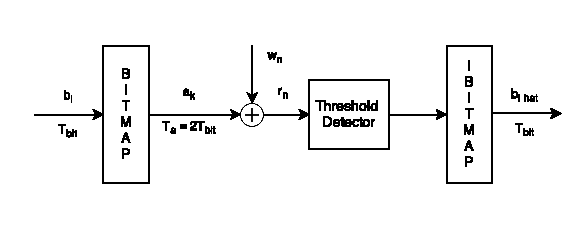
\includegraphics[width = 0.6\textwidth]{SC_uncoded}
	\caption{Block diagram for the simulation of a Single Carrier uncoded QPSK}
	\label{fig:problem1_scuncoded}
\end{figure}

\begin{figure}
	\centering
	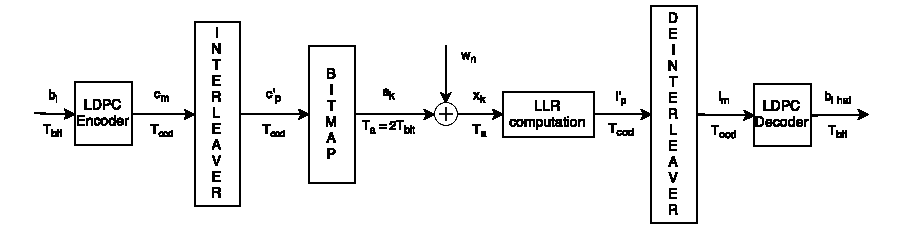
\includegraphics[width = \textwidth]{SC_coded}
	\caption{Block diagram for the simulation of a Single Carrier coded QPSK}
	\label{fig:problem1_sccoded}
\end{figure}

The uncoded Single Carrier QPSK configuration with ideal channel was implemented as described in Figure~\ref{fig:problem1_scuncoded}. First of all, a random data stream is created using the \texttt{randi} function. For the BER simulations, $L_{bits} = 2^{24}$ bits were used for every SNR. While this number of bits is unnecessarily large to estimate the Bit Error Rate for the lower SNRs, it was decided not to optimize it because the simulations were sufficiently fast. This is due to the lightweight operations the script has to perform: after the initial bitmapping of the bits to obtain the QPSK symbols, the channel only adds noise and there is no need to perform any convolution with an impulse response since the channel is ideal. Finally, the receiver only computes a thresholding and an inverse bit mapping. The results of the simulation can be seen in Figure~\ref{fig:problem1_pbit}, and coincide with those obtained in the previous homework. %TODO insert this reference to the old homework???

When using coding, the script has to perform more complex computations that are illustrated in Figure~\ref{fig:problem1_sccoded}. The random bit sequence needs to have a length compatible with both the encoder and the interleaver. In fact, the provided LDPC encoder requires information words to have length $L_{iw} = 32400$ bits, and encodes them into codewords of length $L_{cw} = 64800$ bits. This doesn't represent a limitation, as shorter information words may be padded to reach the desired length, encoded and de-padded at the receiver, once decoded. In order to simplify things, however, it was decided to only send information words that have length that is a multiple of the information word length required by the encoder. Therefore for this problem the number of bits used in order to estimate the bit error probability is $16783200$, which is smallest multiple of the information word length greater than $2^{24}$. 

Additionally, the interleaver matrix was given dimensions of $30 \times 36$ in order to facilitate the process of interleaving the codeword bits. Since $30 \cdot 36 = 1080$ is a divisor of the length of the codewords, when codewords of length $L_{cw} = k \cdot 64800, k \in \mathbb{N^{+}}$ need to be interleaved, the interleaver uses a number of matrices equal to $\frac{L_{cw}}{30\cdot36} = 60 \cdot k$, thus ensuring that all matrices will be filled completely and that no additional padding is required. Using this setup, if the desired length is $L_d$, the nearest compatible length of the message to be sent can be computed using the expression $L_{msg} = \lceil \frac{L_{d}}{32400} \rceil \cdot 32400$. 

Once the bits are generated, encoded and interleaved, they are translated into symbols with $\sigma_a^2 = 2$ using the QPSK bitmap and sent through the channel, that adds the noise $w_k \sim \mathcal{CN}(0, \sigma_w^2)$, given that the SNR of the channel is $\Gamma = \frac{\sigma_a^2}{\sigma_w^2}$. 

The receiver needs then the log-likelihood ratios in order to perform soft decoding. The received symbols are complex, but it is straightforward to extend the definition of LLR proposed in \cite{bc} for the case of binary real symbols in absence of ISI. In particular if the received symbol $x_k = a_k + w_k$ is real, with $a_k$ binary and the noise $w_k$ real Gaussian with variance $\sigma_I^2$, then the log-likelihood ratio LLR is defined in \cite{bc} as 
\begin{equation}
	\ell_k^{bin, real} = \frac{2 x_k}{\sigma_I^2}
\end{equation}
Let's now consider the QPSK case, which is the constellation used by tx-rc in this homework. Note that the bitmap maps the bits with even index ($2k$) to the real part of the $k$-th symbol, the bits with odd index ($2k + 1$) to its imaginary part. Let the received symbol be $x_k = a_k + w_k$, with $a_k = a_{k, I} + j a_{k, Q}$ a QPSK symbol and $w_k$ complex white noise with variance $\sigma_w^2$. Then let $x_{k,I}$ be the real part of $x_k$, i.e. $x_{k,I} = a_{k, I} + w_{k, I}$, with $w_{k,I}$ the noise per component with variance $\sigma_I = \sigma_w^2/2$, and $x_{k, Q}$ the imaginary part, i.e. once again $x_{k,Q} = a_{k, Q} + w_{k, Q}$ with $w_{k, Q}$ with variance $\sigma_I = \sigma_w^2/2$. 

At this point it is possible to define a log-likelihood ratio for the real part and the imaginary part of the symbol $x_k$, which are
\begin{equation}
	\ell'_p =
	\begin{dcases}
	\frac{2 x_{k,I}}{\sigma_I^2}, \quad p = 2k \\
	\frac{2 x_{k,Q}}{\sigma_I^2}, \quad p = 2k +1
	\end{dcases}
\end{equation}

%TODO: more about what the LLR is and on how it works? 

If the symbol period is $T_a$, the LLR vector will have bit period equal to $T_{cod} = \frac{T_a}{2}$, as one value of the LLR corresponds to one bit of the encoded message at the transmitter side. In order to get back to the actual correspondence with the original message $b_l$, it is necessary to deinterleave the LLR and to decode it. By feeding the LLR to the decoder, we are using it in its \emph{soft decoding} mode: the decoder will make use of the likelihood associated to the value of each bit, instead of the ``hard value'' of the bits, to perform the decoding. %TODO Necessary?
The output of the decoder, $\hat{b}_l$, is the final decision on the received symbols. This is the vector that is compared to $b_l$ in order to compute the probability of bit error. The results can once again be seen in Figure~\ref{fig:problem1_pbit}. 

% BER plot for coded vs uncoded QPSK
\begin{figure}
	\centering
	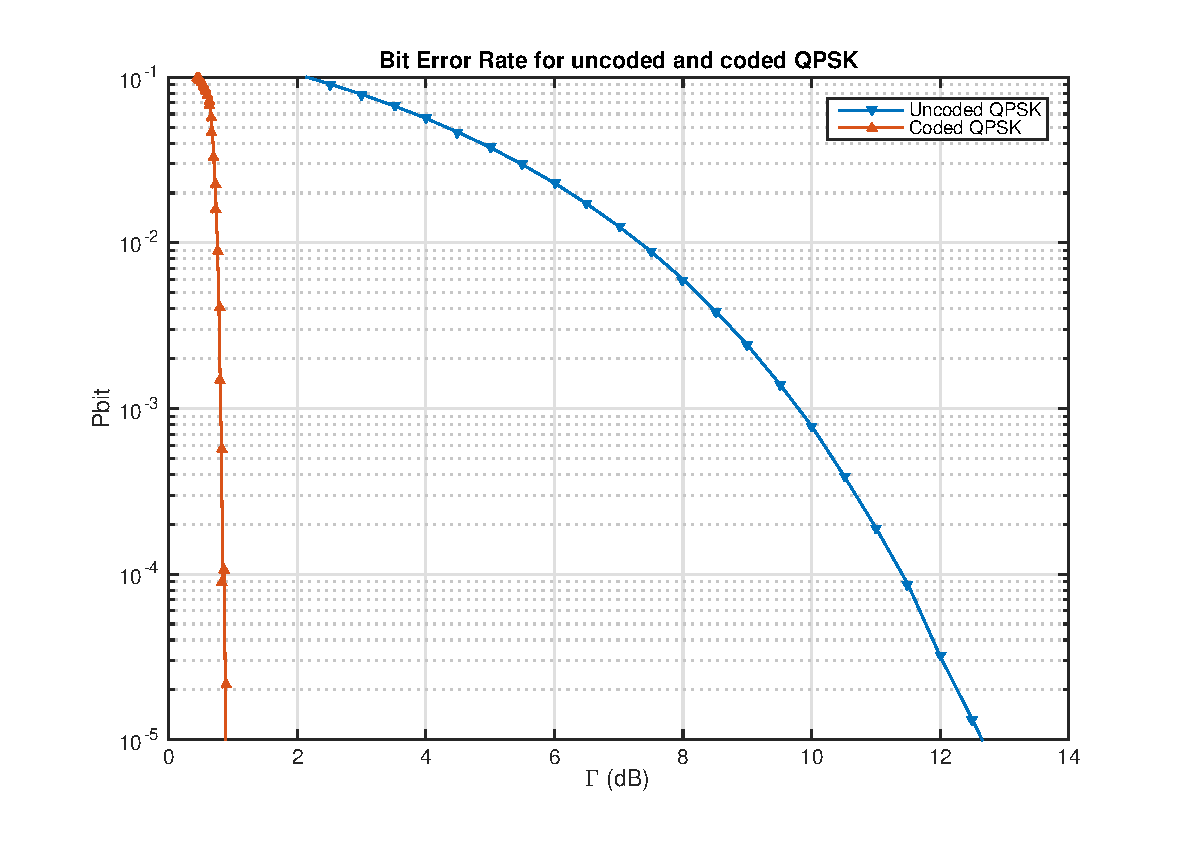
\includegraphics[width = 0.6\textwidth]{problem1}
	\caption{BER simulation results for coded vs. uncoded QPSK}
	\label{fig:problem1_pbit}
\end{figure}

From now on in the Figures that represent the different systems under analysis the coding and decoding blocks will be omitted in order to simplify the description. Therefore a QPSK symbol $a_k$ in the following Figures will represent either uncoded or coded bits. In the first case the symbol $a_k$ is obtained just by applying the bitmap on 2 consecutive uncoded bits. In the second cases, instead, the coding procedure of Figure~\ref{fig:code} is used to encode the bits before the bitmap is actually computed.

\begin{figure}[H]
	\centering
	\subfigure[Coding]{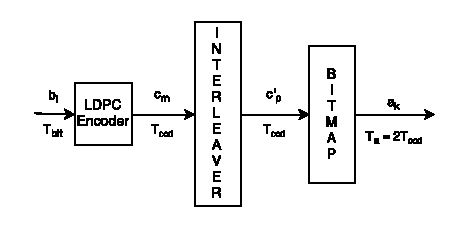
\includegraphics[width = 0.45\textwidth]{coding}}
	\subfigure[Decoding]{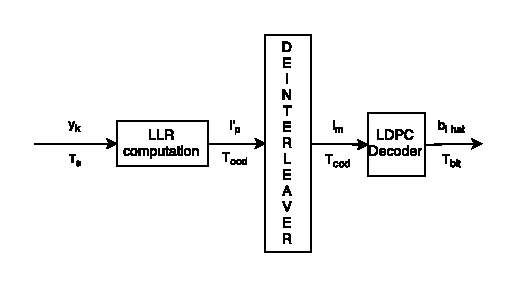
\includegraphics[width = 0.45\textwidth]{decoding}}
	\caption{Blocks for coding and decoding}
	\label{fig:code}
\end{figure}

\FloatBarrier

%%%%%%%%%%%%%%%%%%%%%%%%%%%%%%%%%%%%%%%%%
%%%%%%%%%%%%%% PROBLEM 2 %%%%%%%%%%%%%%%%
%%%%%%%%%%%%%%%%%%%%%%%%%%%%%%%%%%%%%%%%%

\section*{Problem 2}
In order to compute the BER, we need to use two different schemes in case we exploit channel coding or not. If channel coding is used, the DFE scheme depicted in Figure~\ref{fig:DFE_system} is preceded by a series of blocks that code the message and interleave it, as shown in Figure~\ref{fig:code}. At the receiver side, the $y_k$ signal upon which the DFE takes the decisions is then used to compute the \emph{log-likelihood-ratio} and decoded message using the scheme of Figure~\ref{fig:code}. On the other hand, the simulations that do not use channel coding follow the block scheme in Figure~\ref{fig:DFE_system}, where the symbols $a_k$ are the output of a bitmap that maps the input message to QPSK symbols, and the output of the DFE, $\hat{a}_{k-D}$, is then feeded to an inverse bitmap block that translates back the symbols into bits.

\begin{figure}[h!]
	\centering
	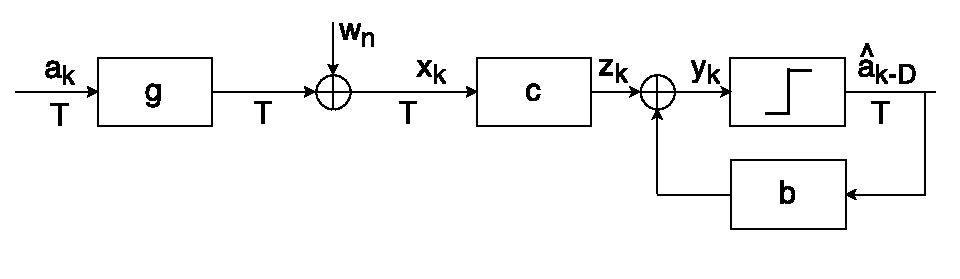
\includegraphics[width = 0.65\textwidth]{DFE}
	\caption{DFE filter}
	\label{fig:DFE_system}
\end{figure}

% TODO Check out the new formulaTION, consider if this should be added:
% Indeed, with this choice the symbol $a_k$ is seen by the receiver as multiplied by the maximum tap of the channel impulse response.
The timing phase is $t_0 = 5 T_a$. Since $t_0$ is defined as the phase offset between the transmitted and received sequence that yields the highest cross-correlation between the two, it was determined as the index for which $|g_i|$ is maximum, which in this case coincides with the first non-zero sample of the channel impulse response ${g_i}$. This choice means that considered the given channel the number of precursors and postcursors we will consider are $N_1 = 0$ and $N_2 = 4$. The SNR of the system is $\Gamma = \frac{\sigma_a^2 E_g}{\sigma_w^2}$, with $\sigma_w^2$ the power of the additive white Gaussian noise of the channel.

% About the DFE
The DFE filter, whose formulation is the same as previous homework, is designed considering the perfectly known channel impulse response and channel noise. The parameters are $M_1, M_2, D$, but $M_2$ is actually dependent on $M_1$ and $D$ because in order to cancel out all the postcursors it must be $M_2 = N_2 + M_1 - 1 - D$. The values of $M_1$ and $D$ chosen are the ones
that minimize the functional $J_{min}$ of the DFE for the lowest SNR $\Gamma$ we are asked to consider, which is $\Gamma = 0$. The choice is then checked against the $J_{min}$ for higher SNR up to 14 dB, and if they are too small, i.e. they do not minimize the functional, they are updated in order to have filters that work in the best way for all the $\Gamma \in [0, 14]$ dB considered. In Figure~\ref{fig:jmin_DFE} the functional $J_{min}$ is plotted against $M_1, D$ for the lowest and highest SNR considered. 
\begin{figure}[h!]
	\centering
	\subfigure[$\Gamma = 0$ dB]{\includegraphics[width = 0.4\textwidth]{JminDFE_0}}
	\subfigure[$\Gamma = 14$ dB]{\includegraphics[width = 0.4\textwidth]{JminDFE_14}}
	\caption{$J_{min}$ for different values of $\Gamma$}
	\label{fig:jmin_DFE}
\end{figure}

The values chosen for the DFE of the receiver are $M_1 = 15, D = M_1 - 1 = 14, M_2 = 4$. These parameters are fixed: they are used both when simulating different SNRs and when supposing the channel to be known or estimated. Instead, the actual coefficients of the filters are computed separately for each simulation, and hence change according to the impulse response and noise variance of the channel (be it the actual ones or the estimated ones).

When the channel estimate is needed, it is performed by sending through the channel a training sequence of $L=31$ binary symbols, partially repeated of $N_{ts} = 7$ symbols. The LS estimate of the channel impulse response and of the noise variance is then used by the DFE to perform the equalization. Note that the estimation is carried out in the same way as in the previous homework, with the exception of the length of the training sequence. 

In the coded case, the samples $y_k$ that are used to compute the \emph{log-likelihood-ratio} are those that the DFE itself uses to perform the decision (see Figure~\ref{fig:DFE_system}). We define $\psi = g * c$ the convolution of the channel impulse response with the FF filter, and $v_k = i_k + n_k$ the total noise, obtained as the sum of the white channel noise $n_k$ and of the residual of ISI term $i_k$. This last term is due to imperfect cancellations performed by the DFE filter and it can be modeled as Gaussian.

Using the previous definitions, the signal at detection point can be expressed as $y_k = \psi_D a_{k-D} + v_k$. Furthermore, recall the definition of functional 
\begin{equation}
 	J = E[|a_{k-D} - y_k|^2] = E[|e_k|^2].
\end{equation}
This allows us to write 
\begin{equation}
	e_k = a_{k-D} - \psi_D a_{k-D} - v_k = a_{k-D} (1 - \psi_D) - v_k.
\end{equation}
Now, if we pick $c = c_{opt}$ (as we actually do, since we compute the FF filter using the Weiner-Hopf method), the functional is minimized, and since the terms $a_{k-D} (1 - \psi_D)$ and $v_k$ are assumed to be uncorrelated, we can write: 
\begin{equation}
	J_{min} = E[|a_{k-D} (1 - \psi_D) - v_k|^2] = \sigma_a^2 |1-\psi_D|^2 + \sigma_v^2.
\end{equation}
Since we are interested in an expression for the noise variance at detection point in the DFE $\sigma_v^2$, we finally find that 
\begin{equation}
	v_k \sim \mathcal{CN}(0, J_{min}-\sigma_a^2|1-\psi_D|^2).
\end{equation}
In order to maintain the receiver QPSK constellation the same as that of the transmitter, we normalize the $y_k$ signal and use:
\begin{equation}
 	 \bar{y}_k = \frac{y_k}{\psi_D} = a_{k-D} + \bar{v}_k, \quad \bar{v}_k \sim \mathcal{CN}\left(0, \frac{J_{min}-\sigma_a^2|1-\psi_D|^2}{|\psi_D|^2}\right).
 	 \label{eq:noisevar}
 \end{equation}

If we set the DFE to use the actual impulse response of the channel and channel noise, we can assume that there is no much ISI left after the cancellation performed using the $b$ filter. Anyway there could be still some wrong decisions which result in erroneous cancellations. Thus, the variance of the noise component of the samples $y_k = y_{k,I} + j y_{k,Q}$ considered in the LLR formula is $\sigma_I^2 = 0.5 \sigma_v^2$, as the per component noise must be considered, with $\sigma_v^2$ as in~\eqref{eq:noisevar}. The LLR formula that is used in this case is then:

\begin{equation}
	\ell'_p =
	\begin{dcases}
	\frac{2 y_{k,I}}{\frac{1}{2} \sigma_v^2}, \quad p = 2k \\
	\frac{2 y_{k,Q}}{\frac{1}{2} \sigma_v^2}, \quad p = 2k +1
	\end{dcases}
	\label{eq:problem2llr}
\end{equation}

In the case of the DFE driven by the estimate of channel impulse response and noise power, the resulting LLR formula is the same as~\eqref{eq:problem2llr}, however the component variance $\sigma_v^2$ this time is different, because the filter coefficients and the functional $J_{min}$ are computed exploiting the imperfect estimation of the channel. This means that also the resulting $\sigma_v^2$ will contain a flawed estimate of the channel noise. 

The results of the simulations can be seen in Fig.~\ref{fig:problem2_pbit}. The number of bits used in these simulations is as in Table~\ref{table:BER_len_DFE} for the uncoded case, while for the coded case the length of the bit sequence is fixed to $4212000$, which is the smallest integer greater than $2^{22}$ that is a multiple of the length of encoder information word. This is a sufficient number of bits to estimate error probabilities up to $10^{-5}$, as requested.

The behavior of the system using channel coding with respect to the uncoded one is similar to what was found in Problem 1 (see Fig.~\ref{fig:problem1_pbit}). As the BER displayed in Problem 1 represents an AWGN theoretical limit it can be seen that with respect to the ideal channel, a DFE equalizing a non-ideal channel needs a SNR about 1.2 dB higher to achieve the same performance if the actual impulse response and channel noise are known, and a SNR more than 2 dBs higher if the channel information must be estimated (with a training sequence of length $L=31$). This applies both to the coded and to the uncoded scenarios. % TODO More on this?
\begin{table}[h!]
	\begin{tabular}{c|c|c|c|c|c|c|c|c|c|c|c|c|c|c|c|c|c|c|c|c}
		SNR $\Gamma$	& 0 & 1 & 2 & 3 & 4 &	5	&	6	&	7	&	8	&	9	&	10	&	11	&	12	&	13	&	14	\\ \hline	
		Bits	& $2^{13}$ & $2^{13}$ & $2^{13}$ & $2^{13}$ & $2^{13}$ & $2^{13}$ & $2^{13}$ & $2^{15}$ & $2^{18}$ & $2^{18}$ & $2^{20}$ & $2^{20}$ & $2^{22}$ & $2^{22}$ & $2^{22}$ \\
	\end{tabular}
	\caption{Length of sequences used to evaluate the BER for the DFE uncoded case}
	\label{table:BER_len_DFE}
\end{table}

% Required stuff:
% Write expressions of LLRs for the known channel, specifying that the noise that is being taken into account is the actual channel noise. There also is no ISI noise as it is assumed to have been canceled by the DFE, specify this!
% Write expression of LLRs for the estimated channel. Specify that we use the estimated channel noise, as it is the only thing the receiver actually knows. 

\begin{figure}[h!]
	\centering
	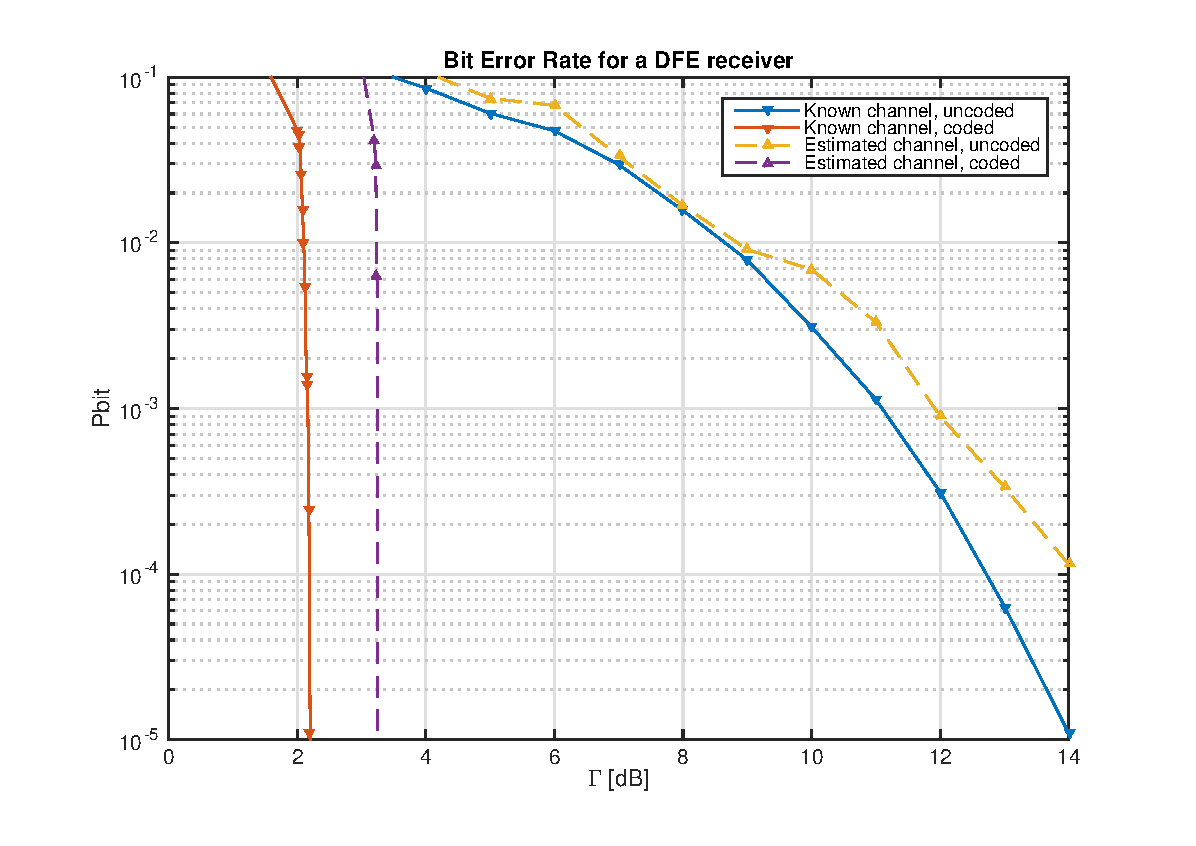
\includegraphics[width = 0.75\textwidth]{problem2}
	\caption{BER simulation for a DFE receiver using the estimated and actual channel impulse response $g_i$, with or without coding}
	\label{fig:problem2_pbit}
\end{figure}

%%%%%%%%%%%%%%%%%%%%%%%%%%%%%%%%%%%%%%%%%
%%%%%%%%%%%%%% PROBLEM 3 %%%%%%%%%%%%%%%%
%%%%%%%%%%%%%%%%%%%%%%%%%%%%%%%%%%%%%%%%%
\section*{Problem 3}

\subsection*{Transmitter structure}
Figure~\ref{fig:OFDM} shows the structure of an OFDM transmitter-receiver and a model for the channel. The symbols denoted by $a_k$ could represent either coded or uncoded bits, as in previous problems. The block index is called $k$. The symbols are taken in chunks of $\ofdM = 512$ in order to compose the vector $a_k[i], i \in [0, \ofdM - 1]$. The IDFT is then computed to get $A_k[i], i\in [0, \ofdM-1]$. At this point a cyclic prefix (whose role will be explained after having introduced the receiver) is inserted, i.e. for each block the last $N_{px} = 7$ symbols are repeated at the beginning of the vector $A_k$. Finally, the symbols $A_k[i]$ are serialized and sent through the channel as part of the signal $s_n$.

\begin{figure}[h!]
	\centering
	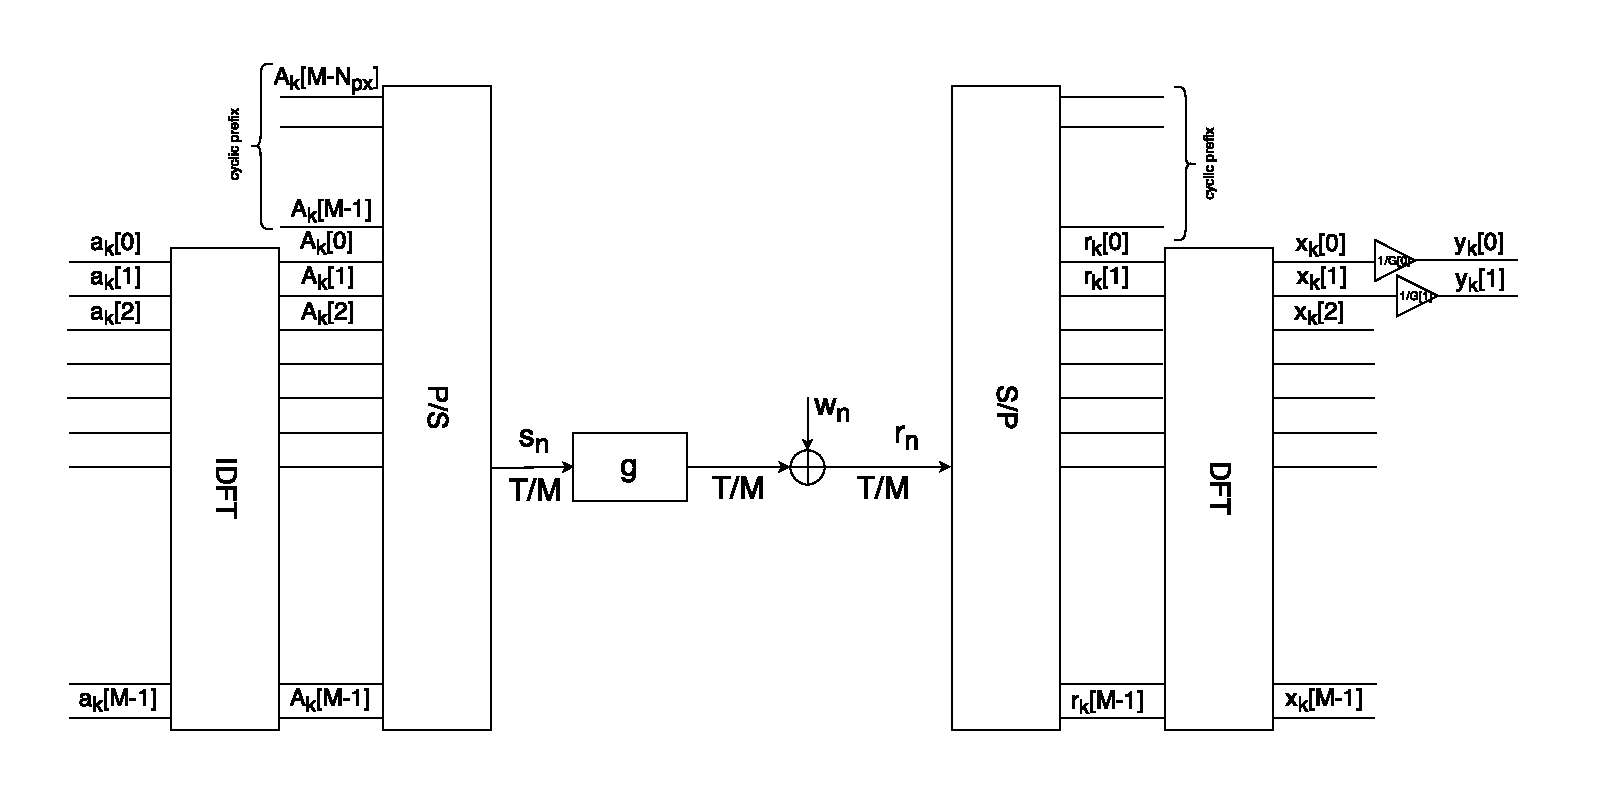
\includegraphics[width = 0.8\textwidth]{OFDM}
	\caption{OFDM system structure}
	\label{fig:OFDM}
\end{figure}
% Consideration on SNR
As usual the SNR is defined as $\Gamma = \frac{\sigma_s^2 E_h}{\sigma_w^2}$, however in an OFDM system the meaning of $\sigma_s^2$ changes. As mentioned, the transmitter performs an IDFT, which is
\begin{equation}
	A_k[\ell] = \frac{1}{\ofdM} \sum_{i = 0}^{\ofdM - 1} W_{\ofdM}^{-i\ell} a_k[i], \quad \ell = 0, 1, \dots, \ofdM-1,
\end{equation}
therefore we have 
% see formula 9.35, 9.38, 9.39
\begin{equation}
	\sigma_s^2 = \dfrac{\sigma_a^2}{\ofdM}.
\end{equation}
To compute the power of the noise introduced by the channel we must then consider the SNR as
\begin{equation}
	\Gamma = \dfrac{\sigma_a^2 E_h}{\ofdM \sigma_w^2},
	\label{eq:snrOFDM}
\end{equation}
which yields
\begin{equation}
	\sigma_w^2 = \dfrac{\sigma_a^2 E_h}{\ofdM \Gamma}.
\end{equation}

\subsection*{Receiver structure}
The structure of the receiver of OFDM is illustrated in Fig.~\ref{fig:OFDM}. The timing phase is $t_0 = 5 T$, and corresponds to the beginning of reception of the cyclic prefix by the receiver. For each block of $\ofdM + N_{px}$ symbols, the first $N_{px}$ are discarded, and the DFT is then computed only on the $\ofdM$ samples that do not belong to the cyclic prefix of that block. Let us define $\mathbf{r}_k$ as the vector of received symbols in block $k$ (before the DFT is performed), $\mathbf{g}_c$ as the channel impulse response of length $N \le N_{px} + 1$, and $\mathbf{g}_{c,\ofdM}$ as the impulse response padded with zeros in order to have a vector of length $\ofdM$. Then it is possible to define the circulant matrix of the IDFT of the transmitted symbols $a_k[i], i = 0, \dots, \ofdM$ as
\begin{equation}
	\boldsymbol{\Xi} = 
	\begin{bmatrix}
		A_k[0] & A_k[\ofdM - 1] & \dots & A_k[1] \\
		A_k[1] & A_k[0] & \dots & A_k[2] \\
		\vdots & \vdots & \ddots & \vdots \\
		A_k[\ofdM - 1] & A_k[\ofdM - 2] & \dots & A_k[0] \\
	\end{bmatrix}
\end{equation}
and express $\mathbf{r}_k$ as
\begin{equation}
	\mathbf{r}_k = \boldsymbol{\Xi} \mathbf{g}_{c,\ofdM} + \mathbf{w}_k
\end{equation}
with $\mathbf{w}_k$ a vector of AWGN samples. %TODO variance? has this w been defined before?
The receiver then performs the DFT using an $\ofdM \times \ofdM$ DFT matrix $\DFTmat$, and since $\boldsymbol{\Xi}$ is a circulant matrix, the result can be written as
\begin{equation}
	 \mathbf{x}_k = \DFTmat \mathbf{r}_k = \DFTmat \boldsymbol{\Xi} \DFTmat^{-1} \DFTmat \mathbf{g}_{c,\ofdM} + \DFTmat \mathbf{w}_k = \mathrm{diag}\{\mathbf{a}_k\} \mathbf{G}_c + \mathbf{W}_k.
\end{equation}
The vector $\mathbf{W}_k$ is a still composed of independent Gaussian random variables, each with variance $\sigma_W^2 = \ofdM \sigma_w^2$. 

This procedure removes the effects of ICI and ISI introduced by the non-ideal channel, and it is followed by a scaling of the received symbols on each channel in order to get the same constellation of the transmitter. More specifically, for each subchannel $i$ we have
\begin{equation}
	y_k[i] = \frac{x_k[i]}{G_c[i]} = a_k[i] + \frac{W_k[i]}{G_c[i]}
	\label{eq:yofdm}
\end{equation}
Finally the receiver performs a decision. If the transmitted bits are uncoded, it uses a threshold detector on each subchannel and an inverse bitmap. Note that the performances of an uncoded OFDM system are negatively affected by the presence of subchannels with a small frequency response coefficient $G_c[i]$. In fact, in those subchannels the received symbols are below noise level, and the noisy term in $y_k[i]$ is amplified by a factor $(G_c[i])^{-1}$.

Instead, if coding is used, the data that would be lost because of the attenuation of its subchannel can be recovered. In particular, given the observed symbol $y_k[i]$ defined in~\eqref{eq:yofdm}, let the variance per component of the noise affecting $y_k[i]$ be
\begin{equation}
	\sigma_I^2 = \frac{\sigma_W^2}{2 |G_c[i]|^2} = \frac{\ofdM \sigma_w^2}{2 |G_c[i]|^2}.
\end{equation}
Then the log-likelihood ratios (LLR) of each subchannel for the pair of bits that are mapped in each symbol are defined as (using $n$ as bit index, since $k$ is the block index):
\begin{equation}
\ell'_p[i] =
	\begin{dcases}
	\frac{2 y_{n,I}[i]}{\sigma_I^2} = 2 y_{n,I}[i] \frac{|G_c[i]|^2 }{\frac{1}{2} \ofdM \sigma_w^2}, \quad p = 2n \\
	\frac{2 y_{n,Q}[i]}{\sigma_I^2} = 2 y_{n,Q}[i] \frac{|G_c[i]|^2 }{\frac{1}{2} \ofdM \sigma_w^2}, \quad p = 2n+1 \\
	\end{dcases}
\label{eq:LLRofdm}
\end{equation}

\subsection*{Channel and noise estimation for OFDM}
In order to perform the operations described in the previous section, the receiver has to know the frequency response of the channel and the noise power of each subchannel. In this homework the simulation of the BER has been carried out both with an \textit{a priori} perfectly known channel and with an estimated channel. 

%TODO give reasons behind this kind of spacing
The estimation of the channel has to be performed with $L_{ts} = 32$ pilot symbols, using one single block, for instance $k=0$. In \eqref{eq:snrOFDM} the power of the transmitted symbols is usually $\sigma_a^2 = 2$, but the pilot symbols have power $\sigma_{ts}^2 = 4$ as required. The pilot symbols $a_{ts}[i]$ are transmitted on the $L_{ts}$ subchannels with indices
\begin{equation}
	i \in \mathcal{T}_{ind} = \left\{q \, \frac{\ofdM}{L_{ts}}, \ q = 0, 1, \ldots,L_{ts}-1 \right\}  = \left\{ 0, 16, 32, \dots, 496 \right\},
	\label{eq:OFDMequallyspacedindices}
\end{equation}
i.e. with a spacing of $\ofdM/L_{ts}$ subchannels between each other. The other $\ofdM - L_{ts}$ symbols can be data or anything else, since they are not used for the estimation. At the receiver, after the DFT, each of the $L_{ts}$ symbols $x_0[i], i \in \mathcal{T}_{ind}$ is divided by the corresponding pilot symbol $a_{ts}[i]$ in order to get $\tilde{G}_c[i]$. Formally, the estimated frequency response of the $i$-th subchannel is
\begin{equation}
	\tilde{G}_c[i] = \dfrac{x_0[i]}{a_{ts}[i]} = \dfrac{a_{ts}[i] G_c[i] + W_0[i]}{a_{ts}[i]} = G_c[i] + \dfrac{W_0[i]}{a_{ts}[i]}, \qquad i \in \mathcal{T}_{ind}.
\end{equation}

Our estimation method exploits the fact that the channel impulse response can have at most $N_{px} + 1 = 8$ taps, so the uncorrelated samples of the frequency response $G_c[i]$ are at most 8. In the presence of noise, however, the estimated frequency response has more than 8 degrees of freedom, and we will try to determine a better estimate (more robust to noise), by using all 32 symbols, equally spaced apart as described above.

Let $\DFTmat$ be a $\ofdM \times \ofdM$ DFT matrix as before, and let $\DFTmat'$ be the result of keeping only the first $N_{px}+1$ columns of $\DFTmat$. Defining $\mathbf{G}_c = [ G_c[i] ]_{i = 0,\ldots,\ofdM-1}$ as the DFT of the channel impulse response, then
\begin{equation}
	\mathbf{G}_c = \DFTmat \cdot \mathbf{g}_{c,\ofdM} = \DFTmat' \cdot \mathbf{g}_c.
\end{equation}
By choosing the 32 subchannels with pilot symbols (i.e. for $ i \in \mathcal{T}_{ind}$) we define a matrix $\DFTreduced$ of size $L_{ts} \times N_{px} + 1$ as the result of selecting the rows $ i\in \mathcal{T}_{ind} $ of matrix $\DFTmat'$. Let 
\begin{equation}
	\mathbf{\tilde{W}} = \left[ \dfrac{W_0[i]}{a_{ts}[i]} \right] _{i\ \in \mathcal{T}_{ind}}
	\label{eq:ODFMnoisevarnormalized}
\end{equation}
be the vector of noise samples corresponding to the considered subchannels (i.e. the ones we are using to transmit the pilot symbols), normalized by the transmitted symbol. Then, defining the vector $\tilde{\mathbf{G}}_c = [ \tilde{G}_c[i] ]_{i\in \mathcal{T}_{ind}}$, it is possible to write $\mathbf{\tilde{G}}_c$ as
\begin{equation}
	\mathbf{\tilde{G}}_c = \DFTreduced \cdot \mathbf{g}_{c} + \mathbf{\tilde{W}}.
	\label{eq:OFDMfreqresp}
\end{equation}

Given an observation of $\tilde{\mathbf{G}}_c $, the vector $\mathbf{g}_{c}$ can be finally computed by applying the LS method, formulated as
\begin{equation}
	\mathbf{\hat{g}}_c = \arg\min_{\mathbf{g}_c} \left|\left|\DFTreduced \cdot \mathbf{g}_{c} - \tilde{\mathbf{G}}_c\right|\right|^2.
	\label{eq:OFDM_LS}
\end{equation}
In matrix form, the solution is given by the following equations:
\begin{align}
	\boldsymbol{\Phi} &= \DFTreduced^H \DFTreduced \\
	\boldsymbol{\theta} &= \DFTreduced^H \tilde{\mathbf{G}}_c \\ 
	\hat{\mathbf{g}}_{c} &= \boldsymbol{\Phi}^{-1} \boldsymbol{\theta}.
\end{align}
Let $\hat{\mathbf{g}}_{c, \ofdM}$ be $\hat{\mathbf{g}}_{c}$ with a zero padding in order to make it $\ofdM$ samples long, as defined before. In order to estimate the frequency response at each subchannel, the DFT is applied on $\hat{\mathbf{g}}_{c, \ofdM}$, to obtain $\mathbf{\hat{G}}_c = \mathcal{F}[\mathbf{\hat{g}}_{c, \ofdM}]$. 
Finally, the noise variance is estimated as 
\begin{equation}
	\hat{\sigma}_w^2 = \frac{\hat{\sigma}_W^2}{\ofdM} = \frac{1}{\ofdM \: L_{ts}} \sum_{i \in \mathcal{T}_{ind}} \left| a_{ts}[i]\hat{G}_c[i] - x_0[i] \right| ^2,
	\label{eq:OFDMestimerror_firstmethod}
\end{equation}
assuming that $a_{ts}[i]\hat{G}_c[i] \! - \! x_0[i]$ has zero mean.

As final remark, to further improve the performance of the system, once $t_0$ is fixed we can truncate the impulse response in order to reduce the degrees of freedom. In fact, the number of postcursors was not dealt with -- i.e. we considered $N_2 \! = \! N_{px} \! = \! 7$. With the notation defined above, we perform the frequency response estimation varying the value of $N_2$ up to $N_{px}$. The estimated noise \eqref{eq:OFDMestimerror_firstmethod}, interpreted as normalized error functional, is plotted versus $N_2$ in Fig.~\ref{fig:OFDM_chooseN2}, that clearly yields $N_2 = 4$ as estimate of the number of postcursors.

Therefore, the rationale above can be developed using $N_2$ in place of $N_{px}$, i.e. allowing only $N_2 + 1$ degrees of freedom for the $\mathbf{\hat{g}}_c$ resulting from the LS problem \eqref{eq:OFDM_LS}. Intuitively, observing that the last $N_{px} \! - \! N_2 \! = \! 3$ samples of $\mathbf{g}_c$ are negligible, we are forcing the channel estimation to yield exactly zero for those coefficients, leading to frequency response and noise estimates closer to the actual values. All results in Problem 3 are obtained with the assumption $N_2 = 4$, and we observed that the estimation is actually improved, as expected. Note that in the following section a different noise estimation is introduced, but for the scenarios at hand they behave in a similar way, thus we will keep the choice $N_2 = 4$ in the next section as well.

\begin{figure}
	\centering
	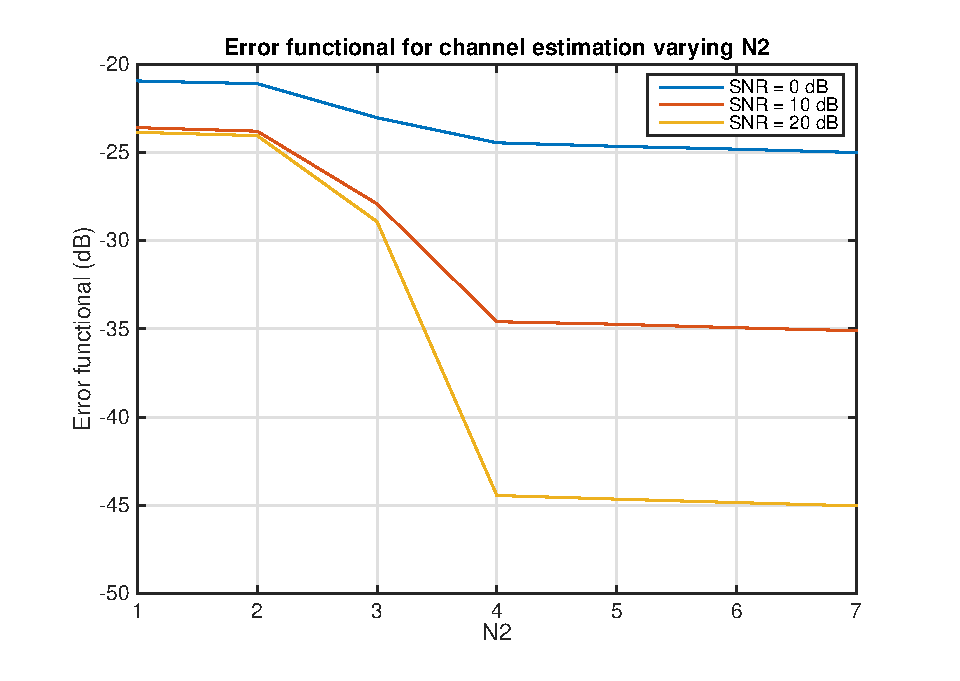
\includegraphics[width = 0.65\textwidth]{OFDM_chooseN2}
	\caption{Estimation error \eqref{eq:OFDMestimerror_firstmethod} for different SNRs, plotted across different choices of the number $N_2$ of postcursors.}
	\label{fig:OFDM_chooseN2}
\end{figure}


\subsection*{Second method for channel and noise estimation}

In absence of noise, \eqref{eq:OFDMfreqresp} can easily be inverted to obtain the exact value of $\mathbf{g}_c$. In fact, that equation represents a system of 32 equations in 8 unknowns, which is an overdetermined system with a unique solution. Actually, we could in principle use any 8 subchannels to get an estimated frequency response -- we tried different scenarios and the resulting estimate is as good as we want, provided a high enough SNR. The presence of noise affects the variance of the estimators: more precisely, the variance of the estimate $\hat{G}_c[i]$, that only depends on the noise, becomes very high for subchannel indices $i$ that are far from the nearest element of the set $\mathcal{T}_{ind}$. For instance, if we use as training subchannels the ones in the middle, i.e. $i = 241,\ldots,272$, then the estimated $\hat{G}_c[i]$ for very low and very high frequencies will be very unreliable. The solution with equally spaced subchannels for the estimation turns out to be the most robust to noise.

As already mentioned, the frequency response we are estimating has only 8 degrees of freedom, therefore in principle we could use for instance 8 equally spaced subchannels to get a good result. Moreover, for the same reason, the 512 coefficients $G_c[i]$ are heavily correlated, therefore adjacent subchannels will have a similar frequency response. The latter observation suggests that a good solution for the estimation of the subchannel noise would be to transmit training symbols on adjacent subchannels, and measure the variance of the estimated frequency responses $\hat{G}_c[i]$, assuming in those subchannels $G_c[i]$ is approximately constant. Indeed, if the noise is powerful enough, the variability of the estimated $\hat{G}_c[i]$ in adjacent subchannels is almost completely due to noise. We chose to consider 8 equally spaced groups of 4 adjacent subchannels each, as explained in the following.

The frequency response estimation in this case is the same as in the first method, except for the index selection -- therefore the resulting estimate will actually be different. A first estimate of the frequency response in 32 indices is performed as in \eqref{eq:OFDMfreqresp}, then the LS problem in \eqref{eq:OFDM_LS} is solved to get $\mathbf{\hat{g}}_c$ and then $\mathbf{\hat{G}}_c$. The difference is in the definition of the $L_{ts}\!=\!32$ chosen indices: the new set of indices is
\begin{equation}
	\mathcal{T}_{ind}^{(2)} = \left\{q \, \frac{\ofdM}{8} + j, \quad q = 0,7, \quad j=0,\ldots,3 \right\}  = \left\{ 0, 1, 2, 3, 64, 65, 66, 67, \dots \right\},
	\label{eq:OFDMnewmethodindices}
\end{equation}
differently from the equally spaced pattern defined in \eqref{eq:OFDMequallyspacedindices}. The frequency response estimation is illustrated in Fig.~\ref{fig:p3_newmethodexample}, in which we show the true response $\mathbf{G}_c$, the estimate $\mathbf{\hat{G}}_c$, and the first raw estimate $\mathbf{\tilde{G}}_c$. The latter vector is shorter than the others, since it consists of $L_{ts}$ elements, which are unevenly placed across the frequency spectrum as per \eqref{eq:OFDMnewmethodindices}.

\begin{figure}
	\centering
	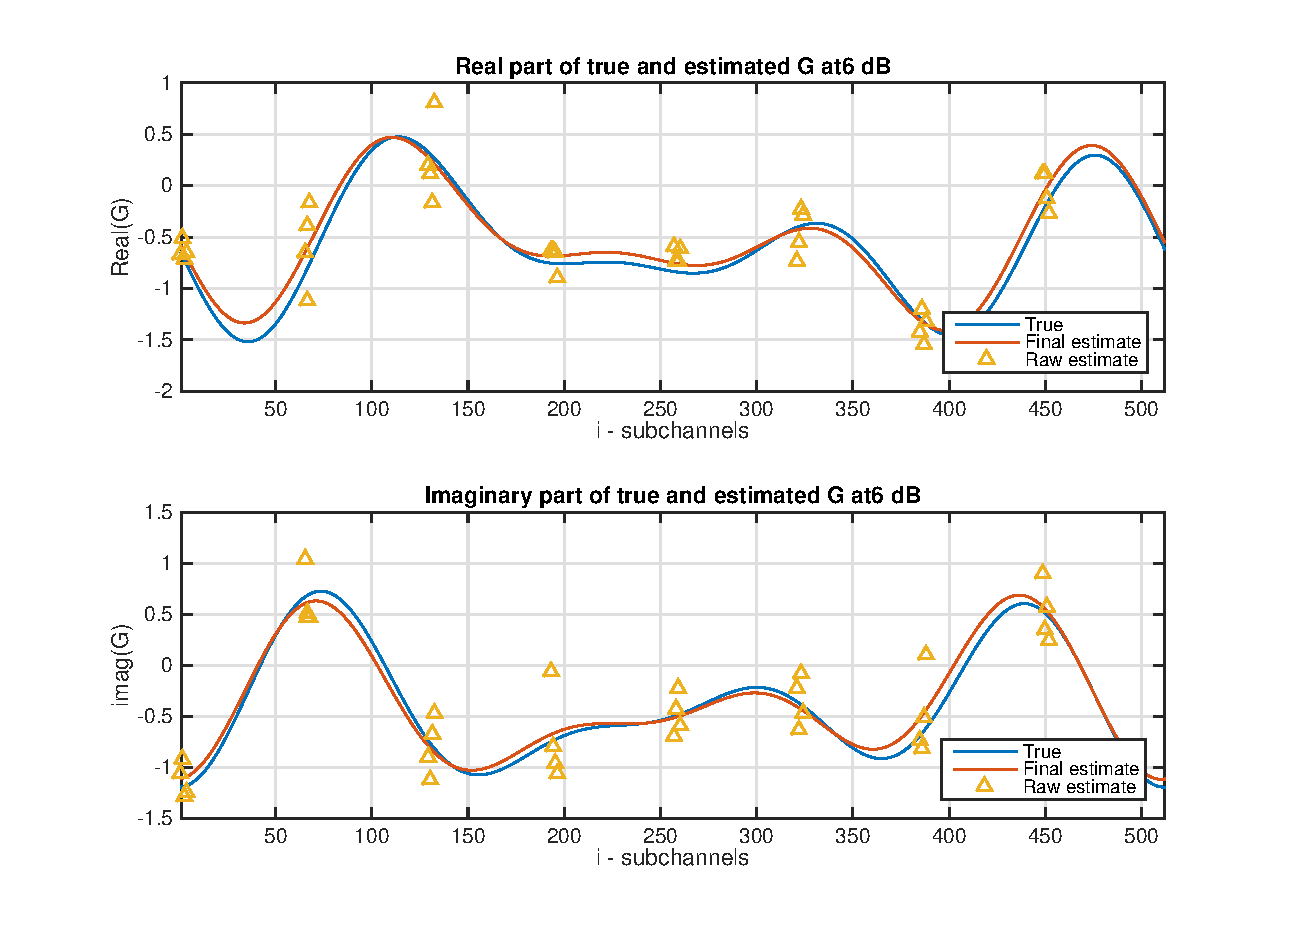
\includegraphics[width = 0.73\textwidth]{p3_newmethodexample}
	\caption{True frequency response $\mathbf{G}_c$, raw estimate $\mathbf{\tilde{G}}_c$ and final estimate $\mathbf{\hat{G}}_c$.}
	\label{fig:p3_newmethodexample}
\end{figure}

As for the noise variance estimation, we proceed as follows. For each of the 8 subchannel groups, we compute the sample variance of the 4 samples and call it $v_q,\ q\!=\!0,\ldots,7$ following the notation in \eqref{eq:OFDMnewmethodindices}. Assuming that in those 4 points the frequency response is the same, as mentioned before, then $v_q$ is an estimate of the variance of the noise $\mathbf{\tilde{W}}$. Looking at \eqref{eq:ODFMnoisevarnormalized} we observe that the variance of $\mathbf{\tilde{W}}$ is
\begin{equation}
	\sigma_{\tilde{W}}^2 = \dfrac{\sigma_W^2}{\sigma_{ts}^2} = \dfrac{\ofdM \: \sigma_w^2}{\sigma_{ts}^2},
\end{equation}
therefore the estimate of the noise variance for a given subchannel group $q$ is
\begin{equation}
	\hat{\sigma}_{w,q}^2 = \hat{\sigma}_{\tilde{W}, q}^2 \: \dfrac{\sigma_{ts}^2}{\ofdM} = v_q \: \dfrac{\sigma_{ts}^2}{\ofdM}.
\end{equation}
Since we have 32 allowed subchannels, and we used the scheme defined in \eqref{eq:OFDMnewmethodindices} for the frequency response estimation, we can iterate the noise estimation on all 8 groups and then take the average, so the estimate of the noise variance is finally
\begin{equation}
	\hat{\sigma}_w^2 = \dfrac{\sigma_{ts}^2}{\ofdM} \left( \frac{1}{8} \sum_{q=0}^{7} v_q \right).
	\label{eq:noisepwrest_newmethod}
\end{equation}

The main tradeoff of this method is the following. Using larger groups of subchannels we are increasing the accuracy of the variance estimation, but there are two downsides. Firstly, the variability of the frequency response starts playing a major role in the estimated variance, yielding a worse estimation of the noise variance, which does not prevail anymore. Secondly, we are increasing the spacing between groups of subchannels, therefore the estimation of the frequency response itself gets worse. On the other hand, using small groups, the estimated variance would be mainly due to noise, and the frequeny response estimation would be more accurate, but we have too few samples in each group to compute the sample variance.

Using 8 groups of 4 subsequent subchannels, the implementation is straightforward, we get a good estimate of the frequency response, and the estimate of the noise power is strongly improved with respect to our original method, up until SNR = 18 dB approximately. With high SNR instead, the estimated variance $v_q$ is given by the local variability of the frequency response $\mathbf{G}_c$ rather than the channel noise. In that case the frequency response estimate is almost perfect, whereas the subchannel noise power will be strongly overestimated since $v_q$ is lower bounded by the local variability of $\mathbf{G}_c$. Some of these performance results are discussed below.

To compare the two methods we tested both of them at different values of SNR. For each SNR, 1000 simulations are performed, in which the channel frequency response and noise power are estimated by mean of the two methods. Hence we consider two performance metrics:
\begin{itemize}
	\item the estimation error on the frequency response $\mathbf{G}_c$ defined as
		\begin{equation}
			\mathcal{E}_G = \dfrac{1}{\ofdM} \sum_{i=0}^{\ofdM - 1} \left| \mathbf{\hat{G}}_c [i] - \mathbf{G}_c [i] \right|^2,
		\end{equation}
	\item the estimated noise variance $\hat{\sigma}_w^2$ with respect to the true $\sigma_w^2$ known \textit{a priori}.
\end{itemize}

Looking at Fig.~\ref{fig:p3_comparison}, the following considerations are in order. As for the first metric, the estimation error on $\mathbf{G}_c$ is the same for the two methods (the 95\% confidence intervals are almost completely overlapped) even though, according to \eqref{eq:OFDMnewmethodindices}, in the second method the training symbols are not sent in subchannels evenly spaced apart.

\begin{figure}
\centering
\begin{minipage}{0.49\textwidth}
\centering
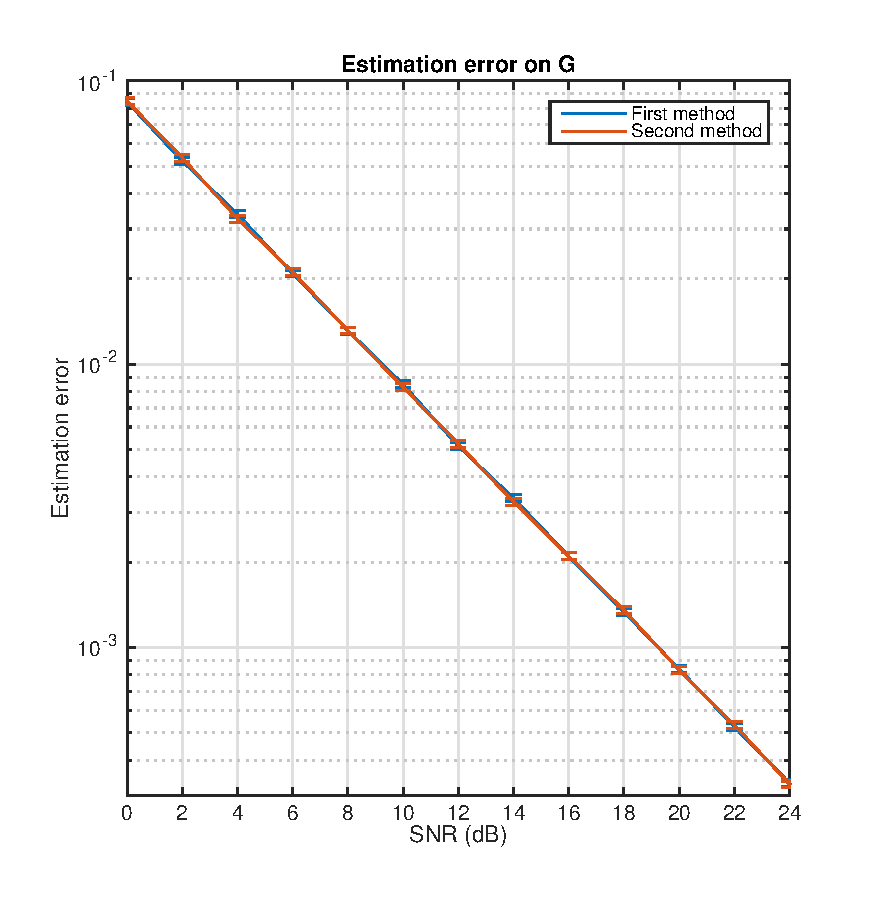
\includegraphics[width=\textwidth]{p3_comparison_estimerror}
\end{minipage}\hfill
\begin{minipage}{0.49\textwidth}
\centering
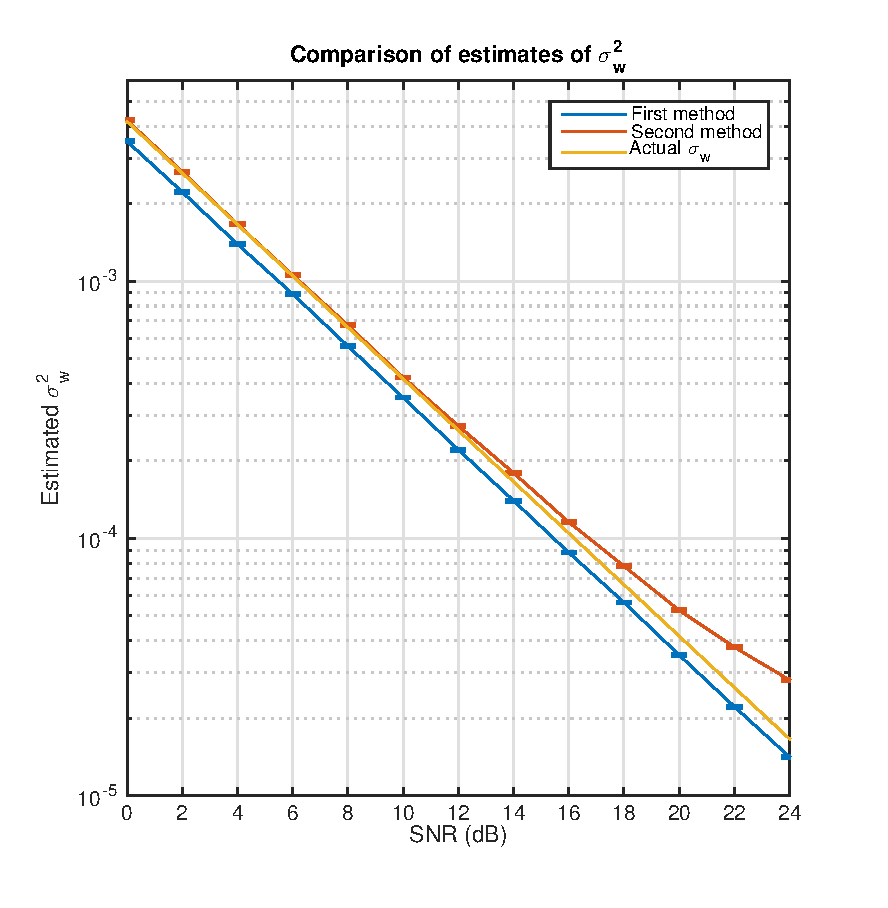
\includegraphics[width=\textwidth]{p3_comparison_noise}
\end{minipage}
\caption{Estimation error on $\mathbf{G}_c$ and estimated noise variance $\hat{\sigma}_w^2$ for the two methods. Mean and 95\% confidence intervals over 1000 simulations. The estimated $\hat{\sigma}_w^2$ is also compared with the actual value of $\sigma_w^2$.}
\label{fig:p3_comparison}
\end{figure}

As for the second metric, the first method always underestimates the noise power. This is due to the fact that some noise is considered as part of the channel response, so its estimated power will be less than the actual one. As a side note, we observed that by increasing the number $L_{ts}$ of training symbols the noise estimation improves: in fact, having more data available, the estimator can more easily distinguish the noise from the useful signal. The underestimation factor is constant for all SNRs.

The second method instead performs much better even with $L_{ts} \! = \! 32$. As we already mentioned, the noise power in this case is overestimated, since the variance $v_q$ we used to estimate the noise in \eqref{eq:noisepwrest_newmethod} considers both the actual channel noise and the local variability of $G_c [i]$. Therefore, for high values of the SNR, the part of $v_q$ that is due to the variability of $G_c [i]$ dominates over the noise variance, and the value of $\hat{\sigma}_w^2$ as the noise power goes to zero tends to a (finite non-zero) number that depends on the variability of $G_c[i]$ around the subchannels chosen in \eqref{eq:OFDMnewmethodindices}.

The overestimation factor of the second method becomes larger than the underestimation factor of the first one when the SNR exceeds 18 dB approximately. Therefore, for the scenarios considered in this homework, the second method proves better than the first one with regards to the noise estimation, whereas the frequency response estimation error is the same, even though the estimated responses are different across the two methods. In conclusion, we chose to apply the second method to the OFDM simulations with estimated channel.

Note that, while the formulation for the LLRs for the OFDM system which uses the channel estimation is the same as~\eqref{eq:LLRofdm}, the variance of subchannel noise used in the log-likelihood ratios of each subchannel is the estimated one, computed from the estimate $\hat{\sigma}_w^2$ of the channel noise given in~\eqref{eq:noisepwrest_newmethod}. Therefore we have that 
\begin{equation}
	\hat{\sigma}_I^2  = \frac{\ofdM \hat{\sigma}_w^2}{2 |\hat{G}_c[i]|^2}
\end{equation}
and
\begin{equation}
\ell'_p[i] =
	\begin{dcases}
	\frac{2 y_{n,I}[i]}{\hat{\sigma}_I^2} = 2 y_{n,I}[i] \frac{|\hat{G}_c[i]|^2 }{\frac{1}{2} \ofdM \hat{\sigma}_w^2}, \quad p = 2n \\
	\frac{2 y_{n,Q}[i]}{\hat{\sigma}_I^2} = 2 y_{n,Q}[i] \frac{|\hat{G}_c[i]|^2 }{\frac{1}{2} \ofdM \hat{\sigma}_w^2}, \quad p = 2n+1 \\
	\end{dcases}
\end{equation}

%%%%%%

\subsection*{BER for OFDM and comparison with DFE}
The results of the simulations for the OFDM bit error rate are in Figure~\ref{fig:BEROFDM}. Note that for the estimated channel just one realization is plotted and that the channel estimation method is the second between the 2 introduced. The number of bits used in these simulations is $2^{22}$ for the uncoded cases, which may be an unnecessary high number but it is justified by the low demand of the OFDM system in terms of memory and computational resources, and $4212000$ for the coded case, as in Problem 2, following the same rationale.

As for the uncoded case, the performances of the system are worsened by the fact that some subchannels exhibit an high attenuation which makes the detection of correct symbols very difficult. Uncoded OFDM does not reach bit error rates below $10^{-3}$ and the BER for the simulation with perfectly known and the one with estimated channel are nearly the same. 

The coded case, instead, performs much better and gets close to the simulated theoretical bound of Problem 1. Indeed, for the perfectly known channel, the steep descent of the BER curve starts at 1.6 dB, while for the estimated channel case it is shifted right of 0.5 dB.
\begin{figure}[h!]
	\centering
	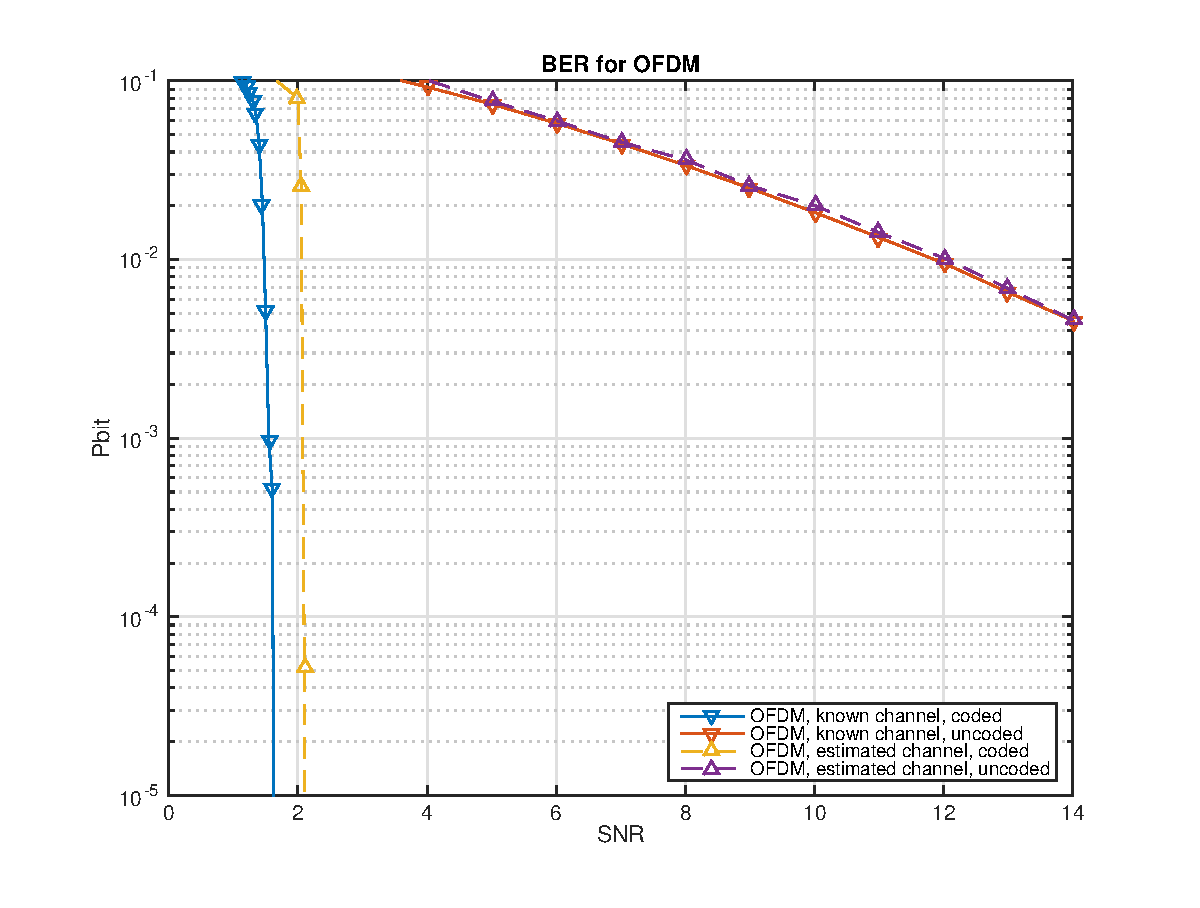
\includegraphics[width = 0.75\textwidth]{OFDM_BER_1}
	\caption{BER for OFDM, coded and uncoded, known and estimated channel}
	\label{fig:BEROFDM}
\end{figure}

Figure~\ref{fig:BEROFDM_comparison} shows instead the comparison between the mean BER of 100 simulations using the 2 different channel estimates, previously introduced in this report. The sample mean of the BER in different simulations can be taken as an estimate of the BER only because the impulse response doesn't change over time, otherwise it would not be meaningful. Note that the errorbars for the confidence intervals are not plotted, otherwise the figure would not be readable. Note also that the non-monotonic behavior can be explained by the fact that 100 simulations are not enough. However the objective of this measures is to show if there is any difference between the performances of an OFDM system in terms of BER when the two different channel estimates are applied. It can be seen that if channel coding is used the BER for the 2 systems is nearly the same, even if the BER of the system with the second channel estimation method for lower SNRs shows a steeper descent and it gains a fraction of dB over the system using the first estimation method introduced. 

If channel coding is not used, instead, the two systems behaves exactly in the same way.
\begin{figure}[h!]
	\centering
	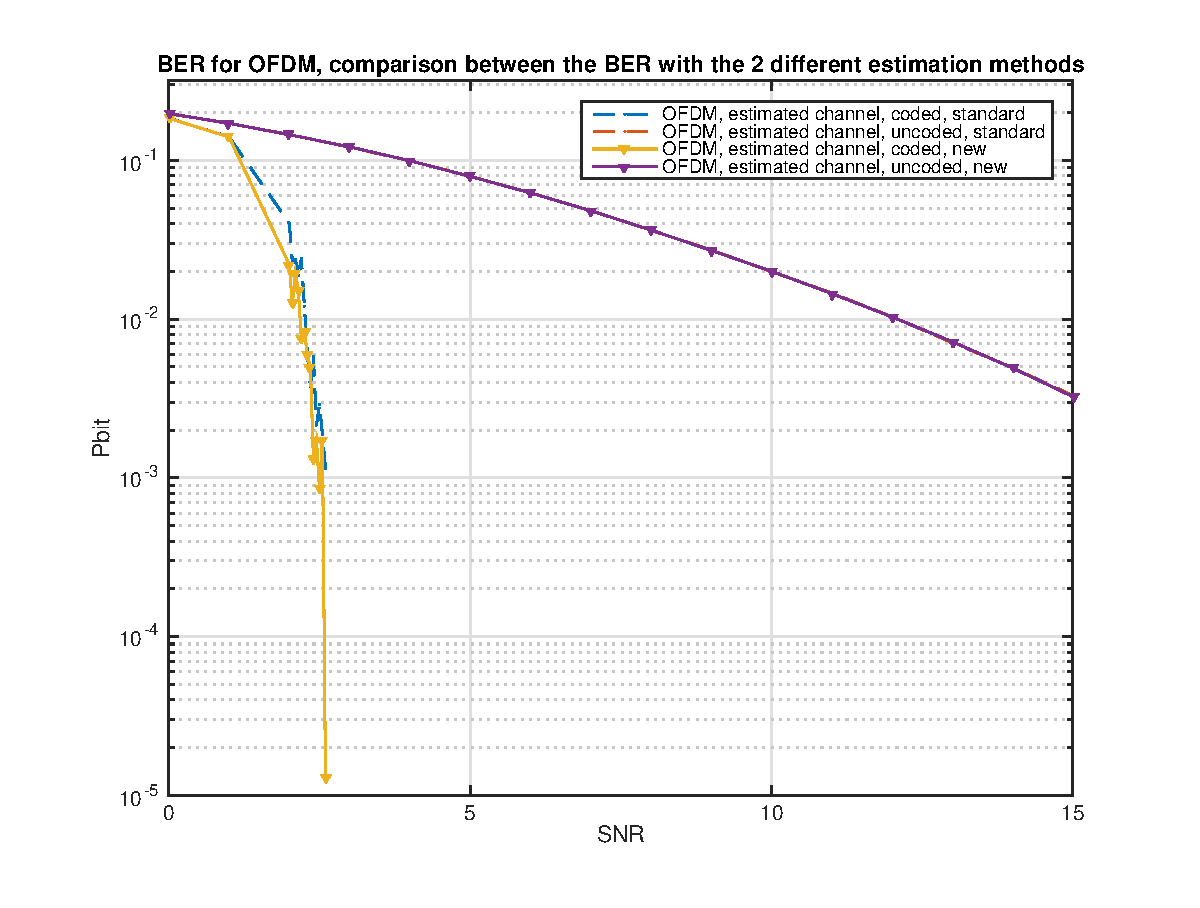
\includegraphics[width = 0.75\textwidth]{OFDM_BER_est_comparison}
	\caption{BER for OFDM, coded and uncoded, using the 2 different channel estimations}
	\label{fig:BEROFDM_comparison}
\end{figure}

The last comparison is between the performances of OFDM and DFE, both coded, with known or estimated channel. The BER curves can be seen in Figure~\ref{fig:DFEOFDM}. Note that in this Figure the values of the SNR $\Gamma$ in the x axis are in $[0, 4]$ dB. Indeed the steep descent that the BER curves present for the coded case happens below 4 dB for all the systems under analysis, therefore it wouldn't make sense to extend it to 14 dB as requested. 

It can be observed that the OFDM, with the known channel, gains about 0.5 dB over the DFE for the same BER. Instead, in channel estimation is used, the OFDM gains about 2 dB. However, the 2 estimation methods are different and the curves plotted are just a single realization, therefore the comparison is less meaningful. However the SNR at which the BER for both systems, with estimated channel, in the different observed realizations is as in Figure~\ref{fig:DFEOFDM}, around 2.1 dB for the OFDM and 3.3 dB for the DFE.

\begin{figure}[H]
	\centering
	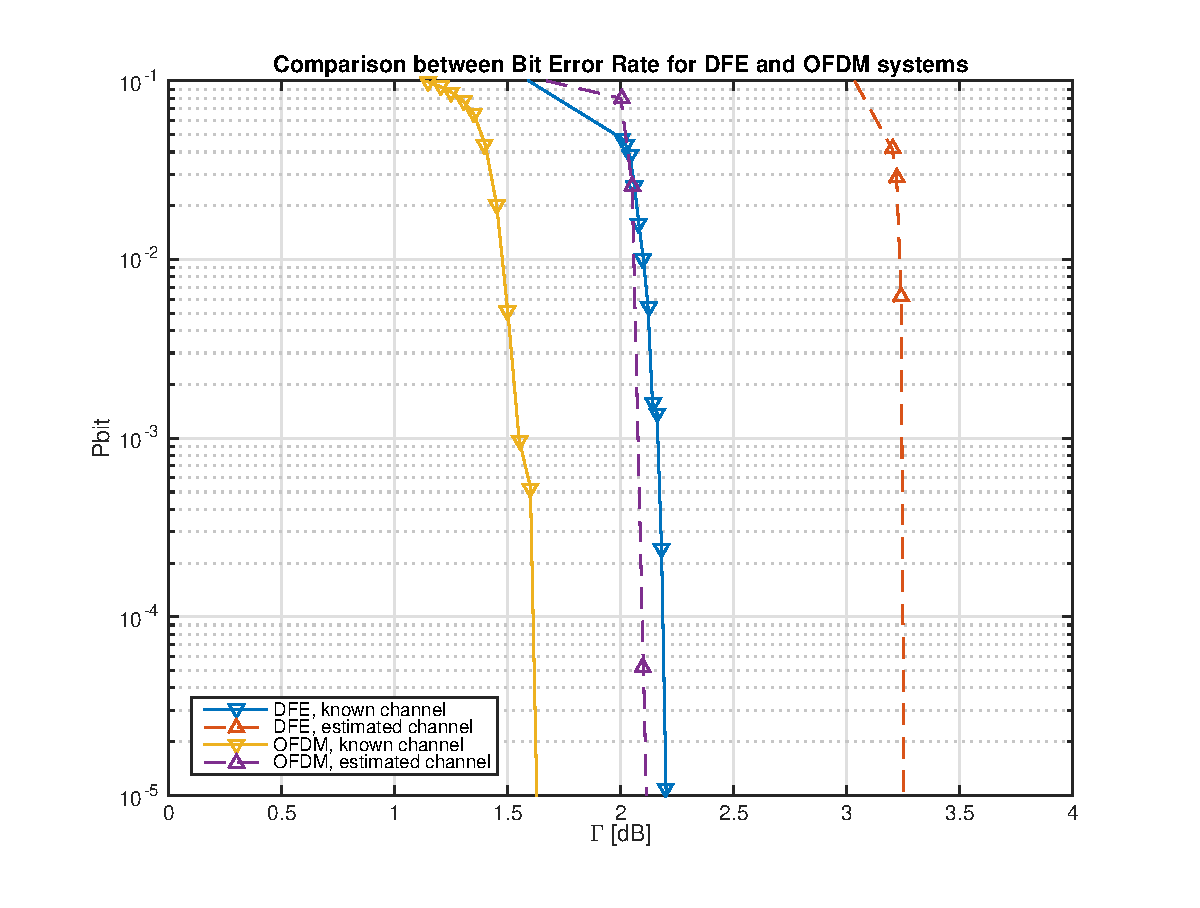
\includegraphics[width = 0.75\textwidth]{OFDMDFE}
	\caption{Comparison between DFE and OFDM, both coded}
	\label{fig:DFEOFDM}
\end{figure}

\FloatBarrier

\begin{thebibliography}{10}

\bibitem{bc}
Benvenuto, Cherubini, Algorithms for Communications Systems and their Applications, Wiley, 2004

\end{thebibliography}

\end{document}
